\documentclass[conference]{IEEEtran}

% Packages
\usepackage{graphicx}
\usepackage{booktabs}
\usepackage{amsmath}
\usepackage{amssymb}
\usepackage{cite}
\usepackage{url}
\usepackage{listings}
\usepackage{xcolor}

% Code listing style
\lstset{
    basicstyle=\ttfamily\footnotesize,
    breaklines=true,
    frame=single,
    language=SQL,
    commentstyle=\color{gray},
    keywordstyle=\color{blue}
}


\lstdefinelanguage{Solidity}{
    keywords={pragma, solidity, contract, function, public, external, view, returns, mapping, struct, event, emit, if, for, while, require, assert, revert, address, bytes32, uint, uint8, uint64, uint256, string, bool, calldata, memory, storage, indexed, indexed, onlyAdmin, onlyPolicyAdmin},
    keywordstyle=\color{teal}\bfseries,
    ndkeywords={function, return, mapping, struct, event, emit, require},
    ndkeywordstyle=\color{brown},
    identifierstyle=\color{black},
    sensitive=false,
    comment=[l]{//},
    morecomment=[s]{/*}{*/},
    commentstyle=\color{gray}\ttfamily,
    stringstyle=\color{red},
    morestring=[b]",
    morestring=[b]'
}


\begin{document}

% Title and authors
\title{Query Performance Analysis of Blockchain-Based Audit Trails for Insurance Access Control}

\author{\IEEEauthorblockN{Anthony Uchenna Eneh $^{1}$, Love Allen Chijioke Ahakonye $^{2}$, Jae Min Lee $^{1}$, Dong-Seong Kim $^{1}$ $^{\ast}$} 
\IEEEauthorblockA{$^{1}$ IT-Convergence Engineering, \textit{Kumoh National Institute of Technology}, Gumi, South Korea \\
$^{\ast}$ NSLab Co. Ltd., Gumi, South Korea,
\textit{Kumoh National Institute of Technology}, Gumi, South Korea}
\IEEEauthorblockA{$^{2}$ ICT Convergence Research Center, 
\textit{Kumoh National of Technology}, Gumi, South Korea}
{(anthony, loveahakonye, dskim, ljmpaul)}@kumoh.ac.kr}
\maketitle


\begin{abstract}
Blockchain-based access control offers tamper-proof audit trails for regulatory compliance, but prior work has not quantified query performance, critical for compliance workflows. We present the first comparison of Ethereum event logs against PostgreSQL and MongoDB for audit queries, benchmarking four patterns (by subject, resource, time range, and denials) across 100--10,000 events. Results show blockchain indexed queries are 6--8$\times$ slower than PostgreSQL while scan-heavy queries are 35--41$\times$ slower, with significantly higher gas costs, trading latency for immutability. These findings inform hybrid architectures: routing critical decisions to blockchain while delegating routine logs to databases.
\end{abstract}

\section{Introduction}
Auto-insurance claims processing involves sensitive evidence across multiple stakeholders, with regulatory frameworks (GDPR, HIPAA) mandating comprehensive audit trails. Compliance officers routinely query these logs: ``Show all unauthorized accesses in Q4'' or ``List accesses to record \#12345.'' Traditional centralized systems suffer from tampering vulnerability \cite{centralized_iam}. ClaimGuard \cite{claimguard_conf}, a blockchain-based ABAC system, addresses this by emitting immutable audit events to Ethereum. Prior work demonstrated authorization correctness but \textbf{never quantified audit log queryability}, a critical gap.

Related work on blockchain audit logging includes BLSQ~\cite{li2024blsq} (Merkle tree optimization without database comparison), BCALS~\cite{bcals2022} (insertion time, not query latency), hybrid blockchain-database benchmarks~\cite{hybrid_bcdb2022} (write throughput only), and VeriBench~\cite{veribench2023} (verification overhead). Blockchain ABAC systems~\cite{oliveira2022smartaccess,ullah2024ehr} lack query benchmarks.

This paper provides the first audit query performance analysis of blockchain-based access control, comparing Ethereum, PostgreSQL 16, and MongoDB 7 across four compliance patterns (100--10K events) with storage cost analysis and hybrid architecture recommendations.

%\section{Related Work}

%Table~\ref{tab:related} compares our work against related approaches. Our work provides the \textbf{first direct comparison} of Ethereum \texttt{eth\_getLogs()} query latency against PostgreSQL and MongoDB for compliance audit patterns---addressing the overlooked dimension of audit \textit{queryability}.

% \begin{table}[t]
% \centering
% \caption{Comparison with Related Works}
% \label{tab:related}
% \scalebox{.8}{
% %\footnotesize
% \begin{tabular}{lccccc}
% \toprule
% Work & \rotatebox{90}{Query Bench} & \rotatebox{90}{DB Comparison} & \rotatebox{90}{Audit Patterns} & \rotatebox{90}{Public Chain} & \rotatebox{90}{Access Control} \\
% \midrule
% BLSQ~\cite{li2024blsq}        & \checkmark &            &            & \checkmark &            \\
% BCALS~\cite{bcals2022}        &            &            & \checkmark &            &            \\
% Hybrid BCDB~\cite{hybrid_bcdb2022} &       & \checkmark &            &            &            \\
% VeriBench~\cite{veribench2023} & \checkmark &           &            &            &            \\
% SmartAccess~\cite{oliveira2022smartaccess} & &          &            & \checkmark & \checkmark \\
% \textbf{This Work}            & \checkmark & \checkmark & \checkmark & \checkmark & \checkmark \\
% \bottomrule
% \end{tabular}}
% \end{table}

\section{System Methodology}

\subsection{ClaimGuard Audit Architecture}

ClaimGuard's audit mechanism consists of an on-chain \texttt{AccessAuditLog} contract emitting indexed events for each access decision:

\begin{lstlisting}[language=Solidity]
event AccessChecked(
    address indexed subject,
    bytes32 indexed resourceIdHash,
    bytes32 indexed actionHash,
    bool allow,
    uint256 ts
);
\end{lstlisting}

The Policy Enforcement Gateway (PEG) calls \texttt{logAccess()} after evaluating policies. Events persist permanently in blockchain transaction logs, queryable via Web3 \texttt{get\_logs()} with indexed filters and block ranges.

\textbf{Query Interface:} Ethereum's event logs support filtering on indexed fields (\texttt{subject}, \texttt{resourceIdHash}, \texttt{actionHash}) and block ranges (\texttt{from\_block}, \texttt{to\_block}). The \texttt{allow} flag is not indexed and requires full log scanning for denial queries.

\subsection{Baseline Systems}

\textbf{PostgreSQL 16:} Traditional relational database with B-tree indexes on \texttt{subject}, \texttt{resource\_id\_hash}, \texttt{timestamp}, and \texttt{allowed}. Partial index on \texttt{WHERE allowed = false} optimizes denial queries. Deployed in Docker (postgres:16-alpine).

\textbf{MongoDB 7:} Document store with indexes on all query fields. Schema validation enforces structure. Deployed in Docker (mongo:7).

Both baselines run on the same hardware as Ethereum (Hardhat local network), ensuring fair comparison.

\subsection{Experimental Design}

\textbf{Event Generation:} We generate 100, 1K, 5K, and 10K synthetic audit events with realistic distributions: 200 unique subjects (Ethereum addresses), 1000 unique resources (evidence items), 6 action types (READ, APPEND, UPDATE, DELETE, ADJUDICATE, DISCLOSE), and 80\% allowed / 20\% denied ratio.

\textbf{Query Patterns:} We evaluate four compliance-driven query patterns. \textit{By Subject} retrieves all accesses by a specific user (e.g., ``What did 0x123... access?'') for compliance audits. \textit{By Resource} identifies all subjects who accessed a specific evidence item for forensic analysis. \textit{Time Range} queries return all accesses within a date window for periodic reporting. \textit{All Denials} filters unauthorized access attempts for security monitoring.

\textbf{Metrics:} Query latency (median, P90, P99 over 10 repetitions), result count, storage costs. We measure end-to-end latency including network overhead (JSON-RPC for blockchain, TCP for databases).

\textbf{Environment:} Hardhat 3.0 (local Ethereum node), PostgreSQL 16-alpine, MongoDB 7 in Docker, same machine (Intel i7, 16GB RAM, SSD). Ensures minimal network variability for local testing.

\section{Results and Discussion}

\subsection{Query Latency Analysis}

Figure \ref{fig:latency} compares query latency across all systems and query patterns at 10K events. Table \ref{tab:latency} reports detailed medians.

\begin{figure}[t]
\centering
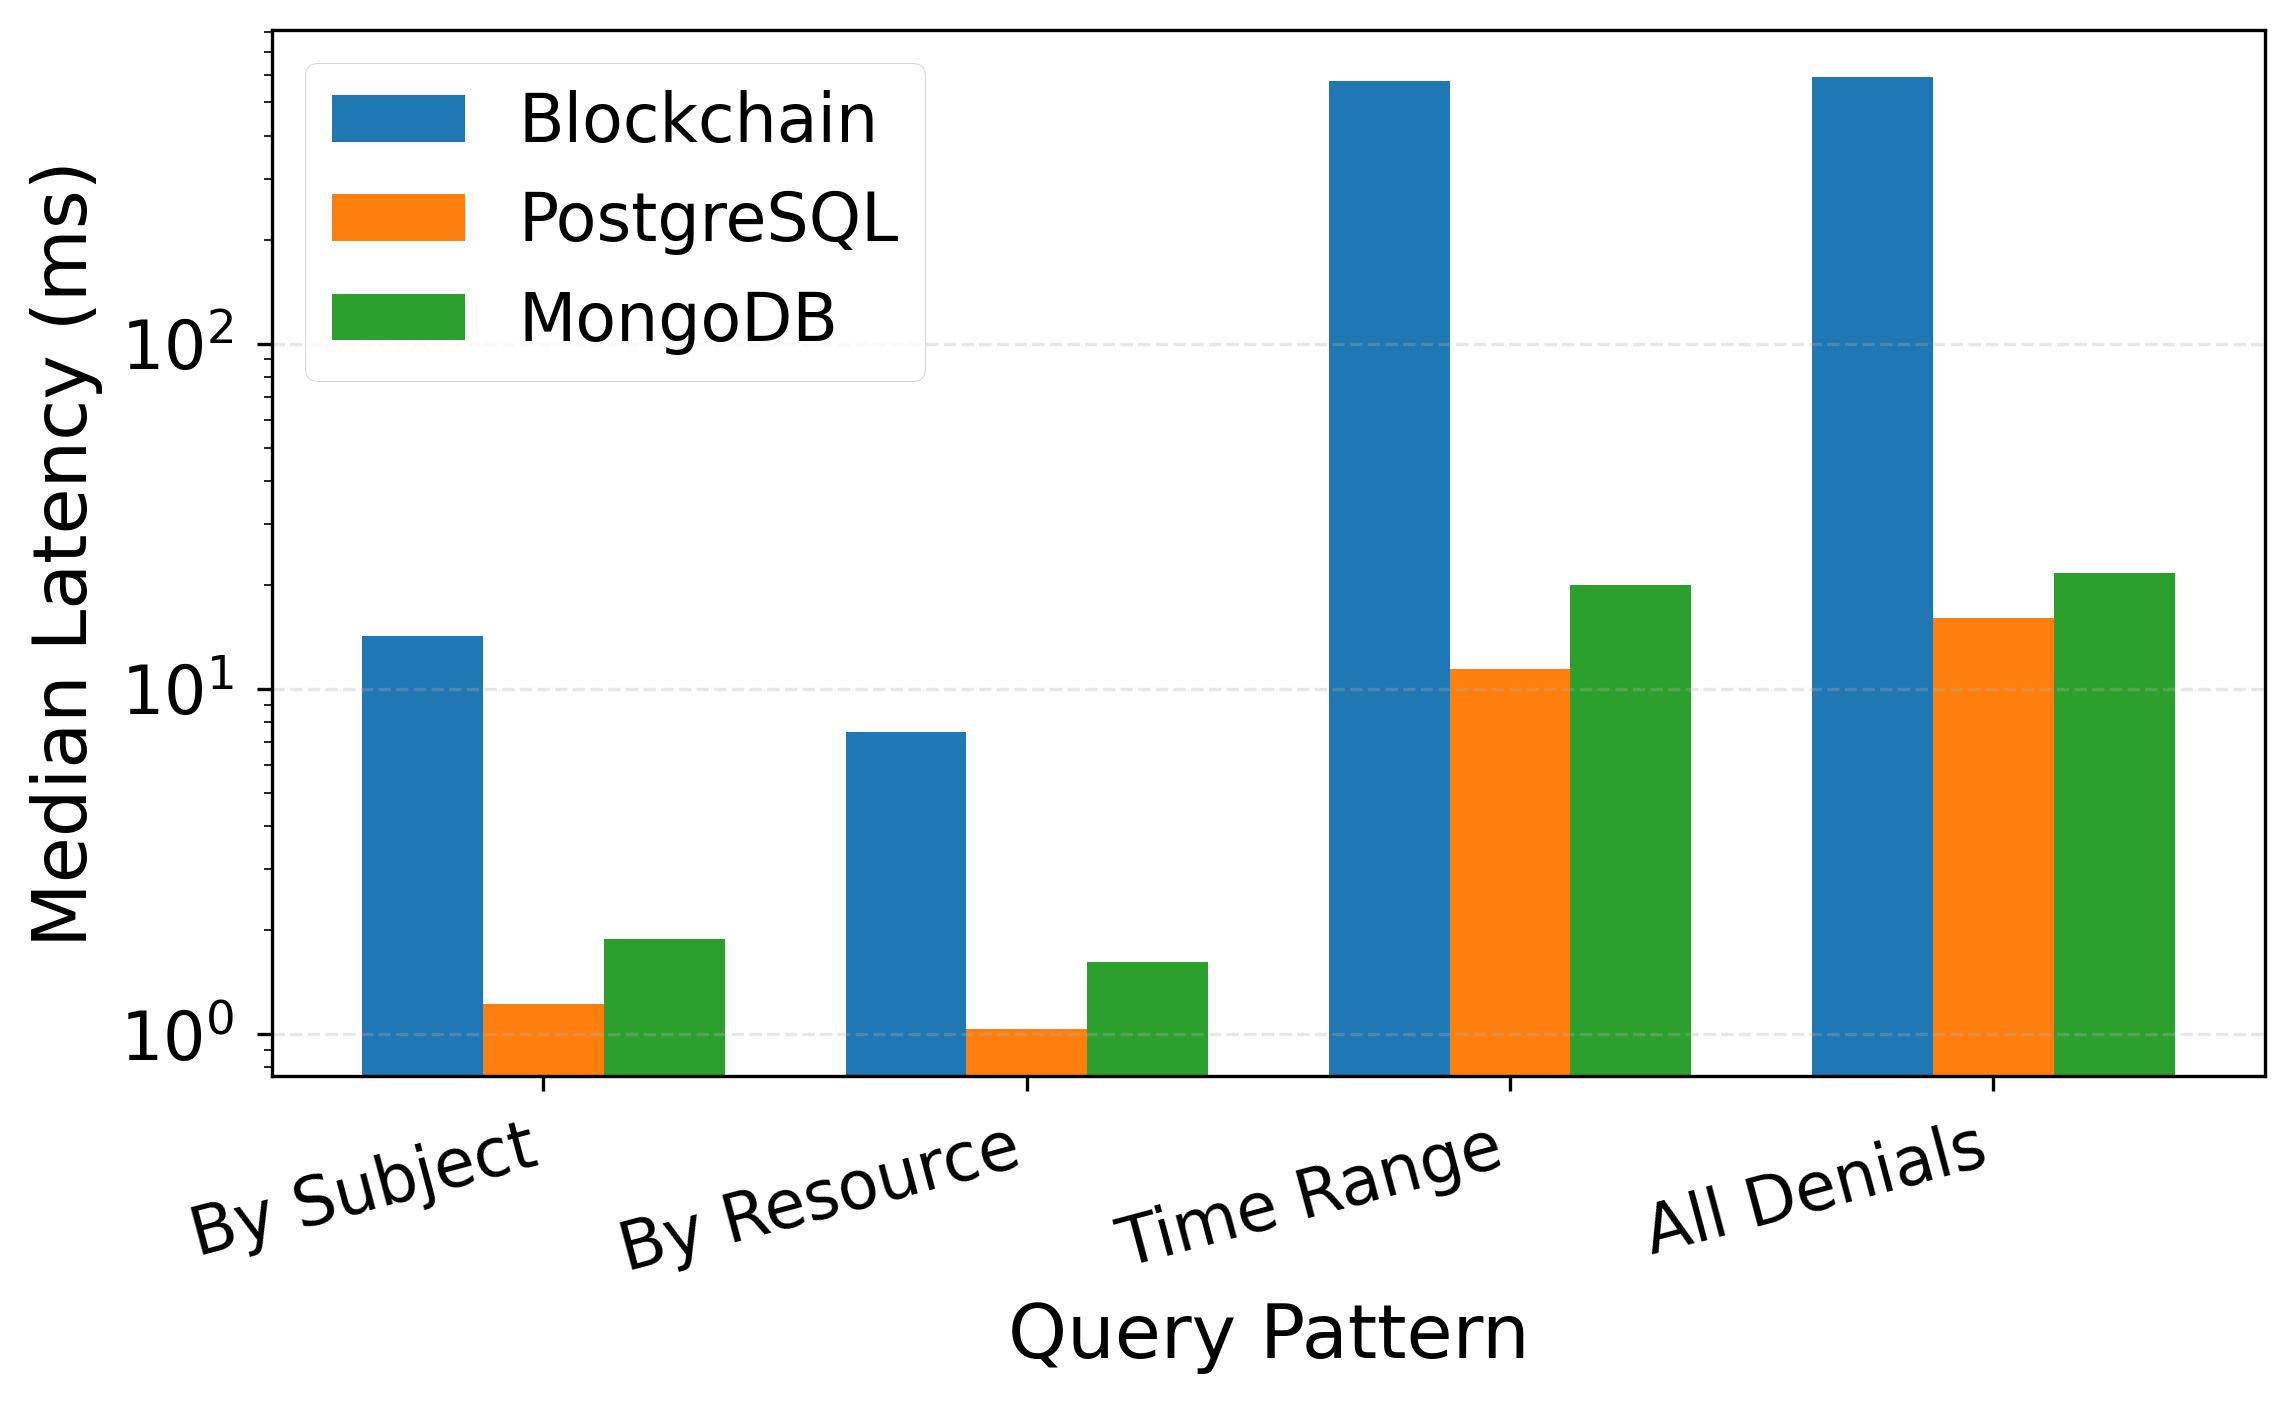
\includegraphics[width=.35\textwidth]{figures/e5_comparison_bar.png}
\caption{Query latency comparison at 10K events. Indexed queries (By Subject, By Resource) show blockchain 6--8$\times$ slower than PostgreSQL. Scan-heavy queries (Time Range, All Denials) show blockchain 35--41$\times$ slower.}
\label{fig:latency}
\end{figure}

\begin{table}[t]
\centering
\caption{Median Query Latency (ms) at 10,000 Events}
\label{tab:latency}
\scalebox{.8}{
\begin{tabular}{lrrrc}
\toprule
Query Pattern & Blockchain & PostgreSQL & MongoDB & Ratio (BC/PG) \\
\midrule
By Subject     &  9.2 &  1.2 &  3.2 &  7.9$\times$ \\
By Resource    &  6.8 &  1.1 &  2.0 &  6.1$\times$ \\
Time Range     & 323.8 &  9.2 & 19.4 & 35.3$\times$ \\
All Denials    & 335.1 &  8.2 & 15.0 & 40.6$\times$ \\
\bottomrule
\end{tabular}}
\end{table}

\textbf{Key Findings:} Indexed queries (by subject/resource) show blockchain 6--8$\times$ slower than PostgreSQL due to JSON-RPC overhead, while PostgreSQL B-tree indexes deliver sub-2~ms lookups. Time-range queries are 35$\times$ slower (323.8~ms vs. 9.2~ms) because block scans cannot leverage timestamp indexes. Denial queries are 41$\times$ slower since \texttt{allow} is not indexed on-chain. Database latency remains stable through 10K events; blockchain scan latency grows with block span.

\subsection{Storage Cost Analysis}

\textbf{Blockchain:} Each \texttt{AccessChecked} event costs $\sim$50,000 gas (event emit + calldata). 10K events $\approx$ 500M gas; at 10 gwei this is about 5 ETH ($\sim$\$10{,}000 at \$2{,}000/ETH). Data persists permanently; retrieval via RPC is read-only but latency is higher for scans.

\textbf{PostgreSQL/MongoDB:} 10K events $\approx$ 1-2 MB disk space, negligible cost. Can be archived/deleted per retention policies.

\textbf{Trade-off:} On-chain Ethereum event storage is orders of magnitude more expensive than database storage due to gas fees---our 10K event benchmark costs approximately \$10,000 on mainnet versus pennies for equivalent database storage. Note this applies to \textit{on-chain} event logs; off-chain decentralized storage (IPFS, Filecoin) offers different economics.

\subsection{Deployment Implications}

Blockchain audit logs are best suited for high-value transactions such as claim settlements and legal disputes, multi-party systems requiring trust minimization, and regulatory scenarios demanding tamper-proof evidence. Databases are preferable for high-frequency low-value accesses, complex analytical queries requiring JOINs, and cost-sensitive deployments. We recommend a hybrid approach: log critical access decisions on-chain while routing routine logs to PostgreSQL/MongoDB, reducing costs 10--100$\times$ while maintaining verifiability for important events.

\section{Conclusion}

We present the first quantitative analysis of blockchain audit log query performance for insurance access control. Testing Ethereum, PostgreSQL, and MongoDB across 100- 10K events, blockchain-indexed queries are 6- 8$\times$ slower while scan-heavy queries are 35- 41$\times$ slower, with gas costs orders of magnitude higher. These findings inform hybrid architectures: routing critical decisions to blockchain while delegating routine logs to databases. Future work includes Layer~2 deployment and off-chain indexing via The Graph.


\section*{Acknowledgment}
This work was partly supported by the Innovative Human Resource Development for Local Intellectualization program through the IITP grant funded by the Korea government (MSIT) (IITP-2025-RS-2020-II201612, 25\%), by the Priority Research Centers Program through the NRF funded by the MEST (2018R1A6A1A03024003, 25\%), and by the MSIT, Korea, under the ITRC support program (IITP-2025-RS-2024-00438430, 25\%) and by the Basic Science Research Program through the National Research Foundation of Korea(NRF) funded by the Ministry of Education (RS-2025-25431637, 25\%).

\bibliographystyle{IEEEtran}
\bibliography{references}

\end{document}
